\chapter{Stabilit\`a locale dei punti fissi}
\begin{definition}[Punto attrattivo/repulsivo]
Un punto fisso $x\in X$ si dice \textbf{attrattivo} se esiste un intorno $U$ di $x$ tale che per ogni $y\in U$ si ha che $\cpa{T^n(y)}_{n\in\N}\subseteq U$ e $\displaystyle\lim_{n\to+\infty}T^n(y)=x$.\\
L'intorno $U$ come sopra \`e un \textbf{bacino di attrazione}.
\vspace{0.25cm}

\noindent
Un punto fisso $x\in X$ si dice \textbf{repulsivo} se esiste un intorno $U$ di $x$ tale che per ogni $y\in U\bs \cpa x$ esiste $n(y)\in\N$ tale che $T^{n(y)}(y)\notin U$.
\end{definition}

\begin{definition}[Semi-attrattivit\`a]
Supponiamo che $X=[0,1]$. Un punto fisso \`e \textbf{semi-attrattivo} o \textbf{semi-repulsivo} se \`e attrattivo da un lato e repulsivo dall'altro.
\end{definition}

\begin{definition}[Orbita attrattiva/repulsiva]
Sia $x$ punto periodico di periodo minimo $p$, allora $\Oc(x)=\cpa{x,\cdots, T^{p-1}(x)}$ \`e \textbf{attrattiva} (rispettivamente \textbf{repulsiva}) se $x$ \`e attrattivo (rispettivamente repulsivo) per $T^p$.
\end{definition}

\section{Punti iperbolici}
\begin{definition}[Punto iperbolico]
Supponiamo che $X\in\cpa{[0,1], S^1, \R, (a,b), [a,b), (a,b]}$ e $T\in C^1(X,X)$. Un punto fisso $x\in X$ si dice \textbf{iperbolico} se $\abs{T'(x)}\neq 1$\footnote{L'idea \`e che $T(y)-x=T(y)-T(x)=T'(x)(y-x)+o(y-x)$, dunque se $\abs{T'(x)}\neq 1$ allora il termine lineare ci dice se per $y$ abbastanza vicino a $x$ vale $\abs{T(y)-x}>\abs{y-x}$ o viceversa.}.
\end{definition}

\begin{proposition}[Relazione tra punti iperbolici e attrattivit\`a]\label{RelazioneTraPuntiIperboliciEAttrattivita}
Sia $T\in C^1(X,X)$ e $x$ un punto fisso iperbolico. Allora 
\begin{align*}
\abs{T'(x)}<1&\implies x\text{ \`e attrattivo}\\
\abs{T'(x)}>1&\implies x\text{ \`e repulsivo.}
\end{align*}
\end{proposition}
\begin{proof}
Studiamo i due casi
\setlength{\leftmargini}{0cm}
\begin{itemize}
\item[$\boxed{\abs{T'(x)}<1}$] Sia $c\in (\abs{T'(x)},1)$ e consideriamo $\delta>0$ tale che $\abs{T'(y)}\leq c$ per ogni $y\in [x-\delta,x+\delta]$. Sia ora $y\in (x-\delta,x+\delta)$, segue che esiste $\xi\in (x,y)$ tale che
\[\abs{T(y)-x}=\abs{T'(\xi)}\abs{y-x}\leq c\abs{y-x}.\]
Segue in particolare che $T(y)\in (x-\delta,x+\delta)$. Ripetendo questo procedimento si ha che $\abs{T^2(y)-x}\leq c\abs{T(y)-x}\leq c^2\abs{y-x}$. Procedendo per induzione
\[\abs{T^n(y)-x}\leq c^n\abs{y-x}\underset{n\to+\infty}{\to} 0,\]
cio\`e $x$ \`e attrattivo con bacino di attrazione $(x-\delta,x+\delta)$.
\item[$\boxed{\abs{T'(x)}<1}$] Sia $c\in (1,\abs{T'(x)})$ e sia $\delta>0$ tale che $\abs{T'(y)}\geq c$ per ogni $y\in [x-\delta,x+\delta]$. Consideriamo ora $y\in (x-\delta,x+\delta)$. Supponiamo per assurdo che $T^n(y)\in (x-\delta,x+\delta)$ per ogni $n$. Con un ragionamento analogo a prima ricaviamo
\[\delta>\abs{T^n(y)-x}\geq c^n\abs{y-x}\underset{n\to+\infty}{\to}+\infty,\]
che \`e assurdo.
\end{itemize}
\setlength{\leftmargini}{0.5cm}
\end{proof}

\section{Criteri per punti non iperbolici}
Risulter\`a utile per alcuni conti la seguente
\begin{remark}[Derivata delle iterate]
Osserviamo che
\begin{align*}
(T^p)'(x)=&\dd x{}\pa{T^{p-1}(T(x))}=(T^{p-1})'(T(x))T'(x)=\\
=&((T^{p-2})'(T(T(x)))T'(T(x)))T'(x)=\cdots\\
\cdots=&\under{=1}{(T^{p-p})'(T^p(x))}\prod_{k=0}^{p-1}T'(T^k(x))=\\
=&\prod_{k=0}^{p-1}T'(T^k(x)).
\end{align*}
In particolare se $x$ \`e un punto di periodo $p$ segue riordinando i fattori della formula sopra che $(T^p)'(T^k(x))=(T^p)'(x)$.
\end{remark}


Supponendo una opportuna regolarit\`a di $T$ possiamo estrapolare il comportamento di alcuni punti non iperbolici. 
\begin{proposition}[Criterio per punti fissi non iperbolici con derivata positiva]\label{CriterioPuntiNonIperboliciDerivataPositiva}
Sia $x_0$ un punto fisso per $T:[0,1]\to[0,1]$ con $T\in C^3$ e $T'(x_0)=1$. Allora
\begin{itemize}
\item se $T''(x_0)\neq 0$ il punto $x_0$ \`e semi-attrattivo.
\item se $T''(x_0)=0$ allora
\begin{align*}
T'''(x_0)>0&\implies x_0\text{ repulsivo}\\
T'''(x_0)<0&\implies x_0\text{ attrattivo}\\
\end{align*}
\end{itemize}
\end{proposition}


\begin{proof}
La dimostrazione segue immediatamente dei seguenti disegni:

\begin{figure}[!htb]
	\centering
	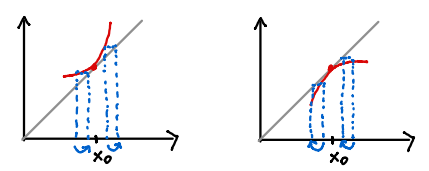
\includegraphics[width=9cm]{Immagini/T''_non_nulla.png}
	\caption{Caso $T''(x_0)\neq 0$. A sinistra il caso di $T''(x_0)>0$ e a destra $T''(x_0)<0$}
\end{figure}

\begin{figure}[!htb]
	\centering
	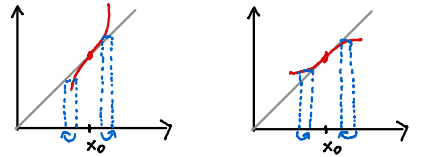
\includegraphics[width=9cm]{Immagini/T'''_non_nulla.png}
	\caption{Caso $T''(x_0)=0$ e $T'''(x_0)\neq 0$. A sinistra il caso di $T'''(x_0)>0$ e a destra l'altro.}
\end{figure}
\end{proof}
	
\begin{definition}[Derivata Schwarziana]
Sia $T\in C^3$, definiamo la sua \textbf{derivata Schwarziana} come
\[ST(x)=\frac{T'''(x)}{T'(x)}-\frac32\pa{\frac{T''(x)}{T'(x)}}^2.\]
\end{definition}
\begin{proposition}[Criterio per punti fissi non iperbolici con derivata negativa]\label{CriterioPuntiNonIperboliciDerivataNegativa}
Sia $x_0$ un punto fisso e sia $T\in C^3$ tale che $T'(x_0)=-1$. Allora
\[x_0\text{ \`e }\begin{cases}
\text{attrattivo} &\text{se }ST(x_0)<0\\
\text{repulsivo} &\text{se }ST(x_0)>0
\end{cases}\]
\end{proposition}
\begin{proof}
Sia $f=T^2$. Poich\'e $x_0$ \`e un punto fisso di $T$ $f(x_0)=T(T(x_0))=T(x_0)=x_0$. Calcolando
\begin{align*}
	f'(x_0)=&T'(T(x_0))T'(x_0)=(T'(x_0))^2=(-1)^2=1\\
	f''(x_0)=&T''(T(x_0))(T'(x_0))^2+T'(T(x_0))T''(x_0)=T''(x_0)-T''(x_0)=0\\
	f'''(x_0)=&T'''(x_0)(T'(x_0))^3+2T'(x_0)T''(x_0)T''(T(x_0))+\\
	&+T''(T(x_0))T'(x_0)T''(x_0)+T'(T(x_0))T'''(x_0)=\\
	=&-T'''(x_0)-2(T''(x_0))^2-(T''(x_0))^2-T'''(x_0)=\\
	=&2\pa{\frac{T'''(x_0)}{-1}-\frac32\pa{\frac{T''(x_0)}{-1}}^2}=2ST(x_0)
\end{align*}
e quindi il segno di $f'''(x_0)$ \`e lo stesso di $ST(x_0)$. Per il secondo punto del criterio precedente (\ref{CriterioPuntiNonIperboliciDerivataPositiva}), $x_0$ rispetta le condizioni di attrattivit\`a o repulsivit\`a volute per $f^2$\footnote{Nel caso della repulsivit\`a questo conclude. Per l'attrattivit\`a notiamo che la convergenza continua a valere per $T$ ma \`e necessario fare attenzione all'intervallo nella definizione di punto attrattivo. La trattazione rigorosa di questo caso non \`e stata data a lezione.}.
\end{proof}

